\question
  Draw all connected graphs of order 5 in which the distance between every two
  distinct vertices is odd. Explain why you know that you have drawn all such 
  graphs.

  \begin{solution}
    Claim that the only graph that satisfies this condition is the complete
    graph. Here it is.

    \begin{center}
      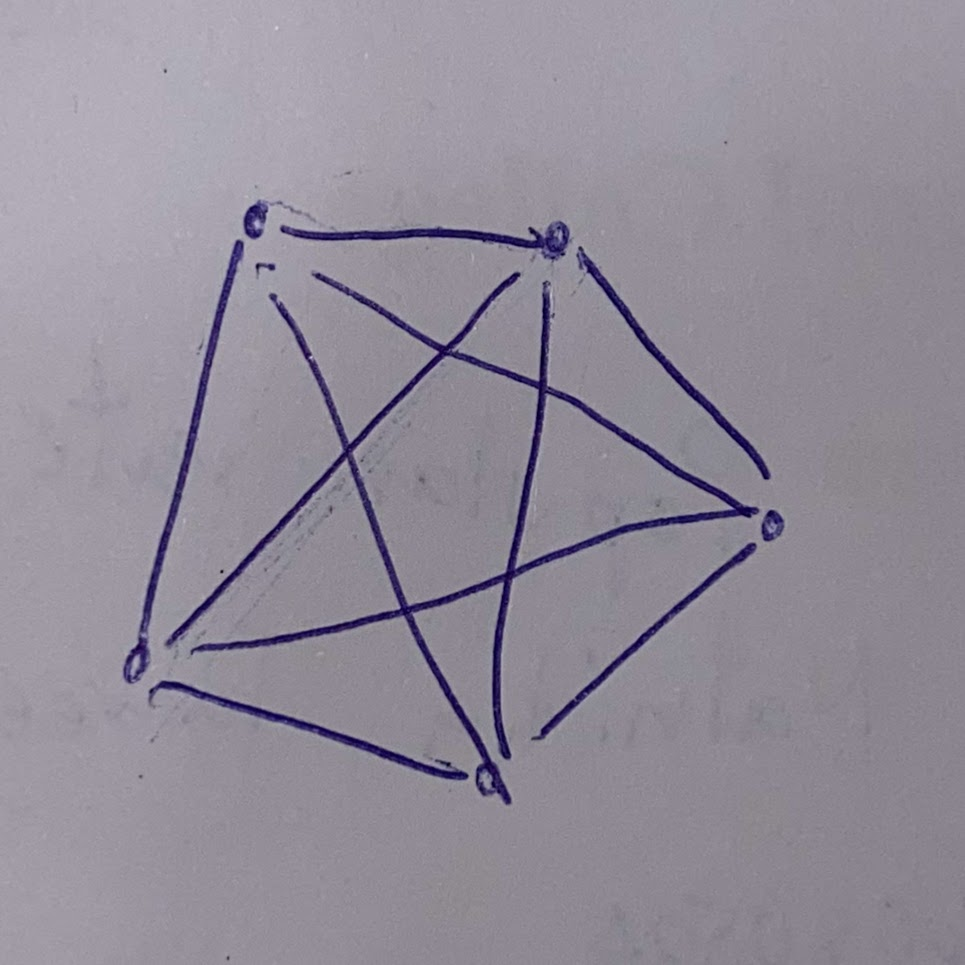
\includegraphics[width=0.31\textwidth]{figures/p1-complete}
    \end{center}

    Now, we claim that if a graph of order 5 satisfies that the distance between
    every pair of two distinct vertices is odd, then said distance must always 
    be 1. This also implies that the graph must be complete since the distance
    between any pair of distinct vertices is 1.

    Assume to the contrary that there exists a pair of vertices \(a, d\) such
    that \(d(a, d) = 3\) and suppose that the path between them is \(a - b - c -
    d\). Then, we would have that \(d(a, c) = 2\) which is a contradiction since
    it has even distance. To reconcile this, we can connect \(a\) to \(c\) to
    make the distance between them 1, but then \(d(a, d) = 2\) through shortest
    path \(a - c - d\), giving rise to another contradiction. Therefore, if 
    every pair of distinct vertices have odd distance, then the distance must
    be 1.
  \end{solution}
